\capitulo{3}{Conceptos teóricos \textit{Scrum}}

Después de analizar diferentes fuentes bibliográfica, se ha decidido tomar como referencia el libro \textit{[Scrum y xp desde las trincheras]}``[Henrik Kniberg, 2018]''\cite{libro} como principal fuente de información.

\section{Introducción}

\textit{Scrum} es una herramienta ágil de trabajo creada por Ken Schwaber, quien defendió que Scrum no era una metodología de trabajo, sino que más bien era un marco de trabajo. Es decir, este sistema explicaba los pasos que se deben seguir para realizar un trabajo con éxito. El autor esclareció que Scrum era un vía a la que adaptarse según la situación concreta en la que se fuera a trabajar, puesto que cada proyecto puede contar con particularidades. De todas formas, el objetivo del libro es desarrollar una forma de trabajo más eficiente y productiva.

En los siguientes apartados pretendemos, analizar el libro, todo ellos desde la visión de la persona que escribió el libro, el sueco Henrik Kniberg.

\section{Cómo hacemos las pilas de producto}

La lista de producto es la parte más importante del \textit{Scrum}. Aquí comienza a funcionar todo el proyecto, en esta lista se incluyen los principales objetivos de los requisitos que se quieren conseguir al final del proyecto, a esto lo llama elementos de la pila o historias.

Elementos de la pila:
\begin{itemize}
	\item \underline{ID}: es el identificador único, contador de los elementos o historias.
	\item \underline{Nombre}: breve explicación del problema a tratar será clara y concisa.
	\item \underline{Importancia}: ratio de consideración que el dueño dé a cada
	elemento.
	\item \underline{Estimación inicial}: valoración del equipo de cuánto trabajo es
	necesario para cada tarea.
	\item \underline{Como probarlo}: realización de pruebas o \textit{demos} en el  \textit{sprint} final, ej.
	realización de pruebas o test.
	\item \underline{Notas}: información que pueda considerarse aclaratoria, o que haga
\end{itemize}

Estos seis campos mencionados son aquellos que más importancia se les da a la hora de realizar los \textit{sprint}. Para la realización de estos campos en los diferentes trabajos académicos es importante realizar los trabajos en tablas Excel, las cuales podrían ver simultáneamente tanto el dueño como los múltiples usuarios.


De la misma manera, el autor menciona que se pueden usar unos elementos adicionales que pueden mejorar la accesibilidad por parte del dueño y así controlarlo mejor las propiedades de cada apartado. Estos campos son: \textbf{la categoría} explicación de la historia básica, \textbf{componentes} realización de tickets para comprobar si los procesos se cumplen, \textbf{solicitante} indicar los avances del producto y \textbf{bug tracking id} seguimiento de errores reportados.

\section{Cómo nos preparamos y planificamos un \textit{sprint}}
Llegados a este punto las preparaciones de los \textit{sprint} se aproximan y lo más importante es tener la pila del producto correctamente lista antes de la planificación del  \textit{sprint}.
Esto quiere decir que es necesario intentar conseguir unos objetivos antes de empezar la
planificación:
\begin{itemize}
	\item Deberá existir la pila del producto.
	\item Habrá una pila de producto y un dueño de producto.
	\item Tendrá los ratios de importancia bien definidos (independientemente de que puedan
coincidir algunos de los ratios para las tareas menos importantes).
 	\item El dueño del producto es el que dará importancia de cada cosa.
\end{itemize}

Una vez concluida la preparación, es momento de desarrollar la planificación, que consiste en realizar una reunión, la que se convertirá en la más decisiva del \textit{scrum}. Si la reunión fuera mal ejecutada podría arruinar por completo el \textit{sprint}, el objetivo de esta planificación de \textit{sprint} es dar al equipo la información necesaria para poder trabajar durante las siguientes semanas.

Los objetivos de la planificación del \textit{sprint} son: establecer la meta, elegir a los miembros con la dedicación que tendrán y realizar la pila del \textit{sprint} (incluyendo las historias). También es adecuado elegir el lugar y la fecha para la reuniones de las celebraciones de los \textit{sprint} diario.

El dueño del producto, por regla, no suele asistir a las reuniones y no trabaja con el equipo, aunque, es recomendable que asista ya que pueden darse tres variables interdependientes, como muestra la figura \ref{triangulo}.

\begin{wrapfigure}{r}{0.4\linewidth}
    \centering
    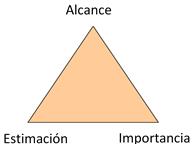
\includegraphics[width=0.30\textwidth]{triagulovariables}
    \caption{Triangulo de variables}
    \label{triangulo}
\end{wrapfigure}

El alcance y la importancia son fijados por el dueño de producto. La estimación la proporciona el equipo de trabajo.

Cuando se planifica el \textit{sprint}, estas variables sufren un desajuste continuo con cada dialogo que se produce cara a cara entre el equipo y el dueño del producto.

En el triángulo antes expuesto faltaría un último elemento que sería la calidad. Esta se subdivide en dos categorías: calidad externa e interna, la primera la perciben los usuarios del sistema y se trata de una interfaz lenta y poco intuitiva, por otro lado, dentro de la calidad interna se encuentran los aspectos no visible al usuario, pero con gran efecto en la mantenibilidad del sistema, como consistencia, refactorización. La segunda es algo alcanzable y la calidad interna es algo que no puede ser discutido.

En las reuniones, el dueño de producto explica cuáles son los objetivos del \textit{sprint} y las historias más importantes a conseguir. El equipo las repasa y las asigna un tiempo estimado de ejecución.

Si el dueño no se presentara a las reuniones, se propondría a alguien del grupo para que desempeñara las funciones de delegado durante las reuniones. Si no surgiera un sustituto, se intentaría asignar un nuevo dueño del proyecto y, por último, se pospondrían los lanzamientos del \textit{sprint} hasta que el dueño esté disponible y pueda asistir a las reuniones.

\subsection{\textbf{Reuniones de planificación de \textit{Sprint} que duran}}

Los \textit{scrum} tienen una duración determinada (\textit{time-boxed}). Cuando una reunión de planificación de \textit{sprint} está llegando al final y aún no están todos los objetivos cumplidos, ¿qué se aconseja hacer? se recomienda la opción de dar la reunión por finalizada. La reunión perdería parte de su utilidad y con esto conseguimos que en la siguiente reunión los \textit{sprint} sean más eficientes y se ofrezca menos resistencia cuando se proponga una duración excesiva.

Se recomienda que las reuniones sean lo más ágiles posible, aunque los sprint largos pueden resultar beneficiosos ya que prestan más tiempo a la detección de errores. Aproximadamente tienen una duración de tres semanas.

\subsection{\textbf{¿Qué historias incluir en un \textit{Sprint}?}}

Al principio de las reuniones se intentan poner unos objetivos en común (historias) con la importancia de cada una de ellas; estas se pondrán en orden de mayor a menor. El grupo de trabajo intentará agrupar el número de historias convenientes según ellos estimen que serán
capaces de realizar en la duración de un\textit{sprint}.

Tendremos la lista de las tareas por realizar en la pila del producto y serán incluidas en la pila del \textit{Sprint}, como se puede ver en la siguiente fotografía.

\begin{wrapfigure}{l}{0.3\linewidth}
    \centering
    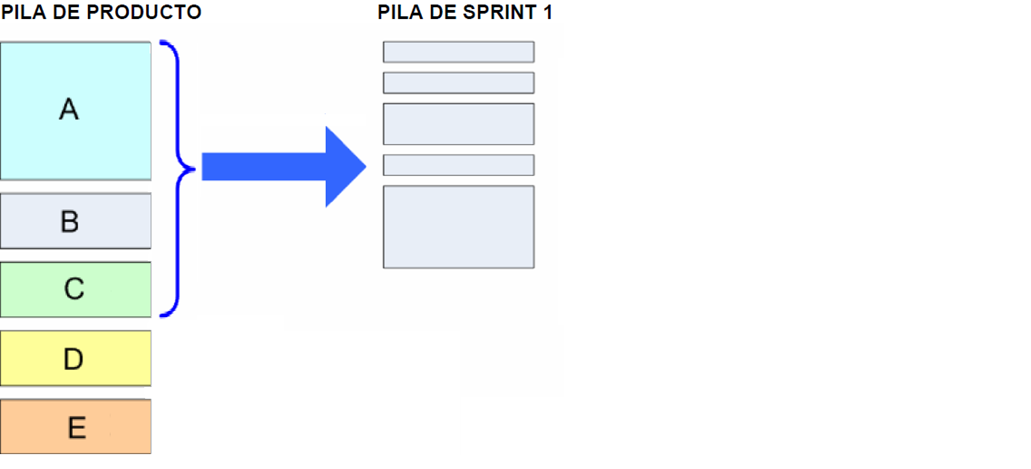
\includegraphics[width=0.45\textwidth]{pasosSprint}
    \caption{Pasos de un \textit{sprint}}
\end{wrapfigure}

En el supuesto de que se quieren meter las tareas A, B y C, pero el dueño del producto quiera introducir la tarea D, una de las posibles combinaciones a realizar es: reorganizar la lista y dejar alguna de las tareas que tenemos fuera. Por ejemplo, nos quedaría A, B y D y se dejaría la tarea C fuera de la pila.

También se podría realizar el reparto de otras formas.\\


El equipo decide qué historias incluir mediante dos cálculos:
\begin{enumerate}
	\item Como se dice tradicionalmente,``a ojo de buen cubero'': suele darse para equipos pequeños y con \textit{sprint} cortos, se calculan suponiendo la dificultad de cada uno de ellos.
	\item Cálculos de velocidad:
	 \begin{enumerate}[a)]
	 	\item \underline{Decir la velocidad estimada}: medida de cantidad de trabajo realizado donde se evalúa en función de la estimación inicial
	 	\item \underline{Calculando las historias que se pueden añadir sin sobrepasar las velocidades}: la velocidad es una medida de cantidad de trabajo realizado, en la cual cada elemento se valora por la estimación que se hizo inicialmente.
	 	Una forma de realizar los cálculos de los recursos será mediante fórmulas, las cuáles son:
	 	\begin{description}
	 		\item [Días – hombre disponible]: Sumaremos los días que emplearan todos los trabajadores del proyecto (días/hombres disponibles).
	 		\begin{enumerate}
	 			\item \underline{Velocidad estimada}:  es igual a la disponibilidad de hombres y días junto al factor de dedicación, que depende de la concentración del equipo. Para calcular un buen factor estudiaremos cómo fueron los anteriores sprint.
	 			\item \underline{Factor de dedicación del ultimo \textit{sprint}}: es igual a la velocidad real repartida entre los días y hombres disponibles.
	 		\end{enumerate}
 		\end{description}
 	\item \underline{Uso de tarjetas}: con este método se logra que todos los integrantes del grupo sean participes y así dar el tiempo de realización de cada actividad.
 	\item Una vez que el equipo tiene definidas todas las tareas, estas se pasarán a una hoja de cálculo  para ver el avance de todo ello.
    \end{enumerate}
	\item Definición de terminado
	
	El primer caso que debe darse para que se considere como acabado es 	que el equipo este de acuerdo con esta decisión. Una historia se considera terminada cuando el encargado del \textit{scrum} así lo determina.
	 
	\item Estimación de tiempos con \textit{PLANNING POKER}
	
	En este tipo de estimación todos los miembros del equipo deben involucrarse para estimar cada historia ya que no sabemos quién implementará cada historia o si esa tarea la realizaran personas de diferentes áreas.
	
	Para ello existe el \textit{planning Poker}, diseñado por Mike Cohn. Esto consiste en cada miembro del equipo cuenta con unas cartas y cada vez que sale una historia los trabajadores tendrán que levantar una carta que indica la estimación del tiempo que necesitaran para realizar ese trabajo. Si los tiempos propuestos son muy diferentes, aquellos que hayan seleccionado las cartas más dispares explicarán sus motivos. Tras ello, se procede a una segunda votación.
	
	Hay dos cartas que son totalmente diferentes a números e indican: ``?'' se desconoce la cantidad de tiempo que puede llevar el desempeño de esta tarea, ``0'' esta historia ya está realizada o apenas lleva tiempo completarla y ``Taza de café'' se solicita un momento descanso.
	\begin{figure}[h]
		\centering
 		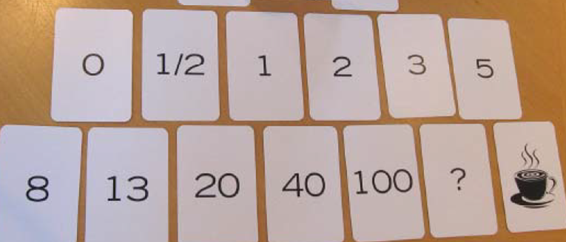
\includegraphics[width=0.7\textwidth]{planningPoker}
 		\caption{Planning poker}
	\end{figure}
	
 	\item Diferencia entre historia y tarea
 	
 	La diferencia es simple, la primera es aquello que se le entrega al dueño del producto; la segunda, los archivos no entregables o aspectos que no preocupan al dueño del proyecto.
 	
 	\item Definir sitio y hora para el \textit{scrum} diario
 	
 	El primer \textit{scrum} es el lanzamiento, cuando decide el personal por dónde empezará a trabajar. Existen dos formas de reuniones:
 	
 	\underline{Por la mañana}, consiste en recordar lo que se realizo el día anterior para ponerlo en común y acordar la tarea a realizar hoy y \underline{por la tarde}, consiste en recordar lo que hemos realizaste durante la jornada de trabajo y hablar sobre lo que realizaras el día de mañana.
 	
 	\item Historias no funcionales
 	
 	Son elementos no funcionales, es decir, son los archivos o elementos no entregables o que no están relacionadas con ninguna historia específica y no tienen mucho valor para el dueño del producto. 
 	
 	Por ejemplo: escribir una descripción del diseño, refactorizar los accesos a los datos o tener un seguimiento de los errores o programa encargado de ello.
	
	\item Seguimiento de errores vs. pila del producto
	
	Hay diferentes programas para el seguimiento de errores. En el libro recomiendan (\textit{Jira}), ya que Excel es un formato bueno para la pila de producto, pero no es tan específico para los errores.
	
	\item Finaliza la planificación del \textit{sprint}
	
	La reunión llega a su fin cuando el dueño del producto y los miembros del equipo llegan a consenso. Una vez que están todos de de acuerdo, el siguiente paso es comenzar a trabajar con un \textit{scrum} diariamente durante las siguientes semanas de trabajo.
\end{enumerate}

\section{Cómo comunicamos los \textit{sprint}}

La comunicación entre la plantilla de trabajo es crucial a la hora de informar sobre lo que está ocurriendo en cada jornada de trabajo. Para informar en todo momento de lo que está sucediendo, en el libro indican que puede ser beneficioso crear una página de información del \textit{sprint}, donde se indiquen los objetivos, pasos a cumplir y fechas de entrega. El jefe del \textit{scrum} podrá imprimir la hoja y dejarla en un lugar visible para que todos los
miembros puedan saber dónde está el \textit{sprint} actualmente.

\section{Cómo hacemos las pilas de \textit{sprint}}

Una vez haya concluido la reunión de planificación del \textit{sprint} y se haya informado a los trabajadores de ello, el jefe del proyecto (\textit{scrum Máster}) debe crear una pila de \textit{sprint}. Esto se hace antes de la reunión de planificación de \textit{sprint}, pero antes del primer \textit{scrum} diario.

El formato de la pila será una lista de tareas, como la imagen que se muestra
a continuación:

\imagen{TablonTareas}{Tablón de tareas}

En dicha tabla se podrán añadir todas las columnas que se deseen, por ejemplo: Test funcionando, proceso cancelado, etc.

El diagrama \textit{burn-down} indicara cómo va el proyecto con respecto al tiempo empleado. (trabajo restante/ fecha estimada).

El gráfico \textit{burn-down} puede indicar varios síntomas:
\begin{itemize}
	\item \underline{Alarmante}: cuando la línea está por encima de la línea de puntos, se considerará quitar elementos de la pila del \textit{sprint}.
	\item \underline{Buen camino}: cuando la línea está por debajo de la línea de puntos, se considerará añadir nuevas historias al \textit{sprint}.
	
\end{itemize}

El \textit{Scrum Máster} es el responsable de asegurarse de que el equipo actúa ante diferentes señales como que se acumulen las actividades en la tarea pendiente o el gráfico \textit{burn-down} no siga una tendencia recta.

\section{Cómo distribuimos la sala del equipo}

Los miembros se reúnen en frente de una pizarra para que se puedan observar entre ellos mientras exponen ideas de cómo abordar los diferentes errores o ideas que puedan surgir durante el devenir del proyecto.

También es importante que los miembros del equipo se sienten juntos o cercanos en el área de trabajo para fomentar la comunicación entre ellos. 

Ventajas de trabajar juntos en la oficina \underline{resultados inmediatos}, \underline{audibilidad} posibilidad de hablar con cualquier miembro del equipo sin levantarse de la silla, \underline{visibilidad} todos los trabajadores pueden ver lo que sucede y tener cercano el tablón de tareas y \underline{aislamiento} mayor orden a la hora de reunir al equipo y no tener que levantarse y molestar a molestar al resto de compañeros de la oficina.

Si el equipo está distribuido, se intentará que este lo más cercano posible usando técnicas como videoconferencia, \textit{webcams}, maquinas remotas de escritorio, etc.

Sería recomendable que el dueño del producto esté cerca para consultar dudas y el tablón de tareas, pero no lo suficientemente cerca de estar al lado del equipo, ya que puede que no sea capaz de controlarse y pueda interrumpir en cualquier detalle y provocar que el equipo no fluya adecuadamente.

\section{Cómo hacemos los \textit{scrums} diarios}

Deben ser realizados todos los días, a la misma hora y en el mismo lugar. Se suelen realizar de pie para intentar que no sobrepasen los 15 minutos de duración. Una vez realizado el \textit{scrum}, actualizamos el tablón de tareas de acuerdo con las indicaciones de los trabajadores sobre lo que realizaron el día anterior y los planes que tienen para ese día. Lo puede realizar el \textit{Scrum Máster} y así, mientras los trabajadores lo indican, él va modificando los \textit{post-it} en el tablón, para incentivar que la gente no llegue tarde, en el libro recomienda el uso de pequeñas multas para que no haya informales en el grupo de trabajo.

\section{Cómo hacemos la \textit{demo} de \textit{\textit{sprint}}}

Tener que hacer una demostración con cada final del \textit{sprint} obliga al equipo a poder demostrar el trabajo realizado durante ese proceso, esto es favorable ya que consigue un \textit{feedback} entre las partes interesadas en el proyecto. Con esto se intenta conseguir un reconocimiento a los trabajadores y las personas que no son parte del proyecto sea capaz de entender lo que realiza el equipo si las demostraciones son claras y descriptivas, estaremos consiguiendo un ahorro de trabajo para futuro trabajo.

\section{Cómo hacemos las retrospectivas de \textit{sprint}}

Las retrospectivas son importantes, en vista de que con ello conseguimos y nos aseguramos de que son realizadas por el equipo. Permite, además, mejorar ideas o alguna cosa que el grupo vio mal en el anterior \textit{sprint}, con el objetivo de que no se vuelva a repetir de nuevo en los posteriores \textit{sprint}.

El autor indica un ejemplo para realizar las retrospectivas:

\begin{itemize}
	\item Reservar de una a tres horas, dependiendo la discusión.
	\item Los representantes: el dueño del producto y el equipo.
	\item Intentar que sea una reunión cómoda y sin gente interrumpiendo.
	\item Designar un secretario.
	\item Intentar que participe todo el mundo, opiniones, errores e ideas sobre el próximo \textit{sprint}.
	\item Observar los tiempos reales con los que teníamos estimados.
\end{itemize}

Se puede escribir sobre una pizarra las retrospectivas con tres columnas: \textbf{buena}, si volviéramos a realizar esta tarea, realizaríamos los mismos pasos, \textbf{mejorable}, ¿qué cambiaríamos si lo volveríamos a realizar las mismas personas? y \textbf{mejoras}, ideas concretas sobre qué mejorar en el futuro.

Se podría decir que \textit{bien} y \textit{mejorable} son miradas al pasado y \textit{mejoras}, miradas al futuro.

\section{Descansos entre \textit{sprint}}

Como indica el libro, no se puede estar siempre esprintando ya que acabarías derrotado y al final estarías haciendo \textit{footing}.

Los \textit{sprint} son muy intensos y por ello hay que dejar espacio entre ellos. Con esto se consigue liberar la cabeza y, \textit{a posteriori}, aportar mejores ideas.

Es conveniente que la retrospectiva y la siguiente reunión no tengan lugar en el mismo día y es incluso aconsejable realizarla con el fin de semana de por medio.

Un de las mejores ideas que propone es tener un día de laboratorio (que los trabajadores puedan tener momentos largos de libertad) para poder realizar otras cosas relacionadas con el trabajo, pero no con ese trabajo, esta idea está inspirada en Google.

%\imagen{DescansosEntreSprint}{Descansos entre \textit{sprint}}

Lo más importante es que entre \textit{sprint} y \textit{sprint} haya horas de desconexión y te permitan dormir para relajarte.

\section{Planificación de entregas y los contratos de precio fijo}

En algunas ocasiones, cuando el contrato es de precio cerrado, necesitamos planificar los \textit{sprint} con antelación. Por ello el propietario necesita las estimaciones aproximadas de las tareas que se incluirán en el contrato, estas tareas las deberá haber realizado con antelación el equipo de trabajo. 

\subsection{Definir los umbrales de aceptación y estimar elementos importantes}

Los umbrales son una clasificación según la importancia de la pila de producto de acuerdo con los términos que aparezcan en el contrato. Conforme con dónde esté el umbral de aceptación, meteremos esto en las diferentes versiones de nuestro proyecto.

Para estimar los elementos más importantes, se deben incluir todas las historias que se añaden en el contrato. Las estimaciones las tendrá que realizar el equipo y no tendrá que dedicarse demasiado tiempo para ello, son estimaciones no compromisos.

\imagen{estimacionElementos}{Estimación de los elementos}

Después de realizar cada \textit{sprint} comprobaremos la velocidad real del \textit{sprint} y, en caso de que sea muy diferente a la que se estimó en un principio, revisaremos la velocidad que dijimos en el resto del \textit{sprint} y tendremos que actualizar el plan de entregas. Quizás la modificación de las entregas no guste al cliente, pero lo que se intenta es cumplir el objetivo y ser honestos con él.

\section{Cómo combinamos \textit{Scrum} con XP}

Hay que indicar que tanto \textit{scrum} como XP (Programación eXtrema) se combinan de forma perfecta, dado que \textit{scrum} se centra en prácticas de organización y gestión, mientras que XP se centra en prácticas de programación. Ya que tratan áreas diferentes pueden complementarse muy bien entre ellas.

Los beneficios de la programación por parejas son:

Mejorar la calidad del código, la concentración, la distribución del conocimiento entre el equipo, poder cambiar de parejas para aportar nuevas ideas, poder estandarizar el código(esto puede ser útil si se cambia de parejas).

El desarrollo guiado por pruebas TDD es un test automático, en el cual tú escribes el código necesario para pasar ese test y a continuación refactorizas el cogido para su legibilidad y eliminar posibles duplicaciones.

TDD es duro, puede llevar tiempo comprenderlo, pero es muy importante, tiene efecto positivo en el diseño del sistema además tiene pruebas de integración tipo ``caja negra'' y permite utilizarlo con otros programas como \textit{Jetty}, Cobertura (métricas).

Una parte importante es el diseño incremental. Consiste en mantener el diseño simple desde el momento que empezamos el proyecto e ir mejorándolo continuamente, posteriormente se podrá limpiar el código y revisarlo. Primeramente, es necesario que funcione de forma correcta, las mejoras del diseño son efectos del realizar el TDD.

Es importante la integración continua, con esto evitamos el problema de que el proyecto funcione en todas las maquinas. Una vez compilado en un ordenador, realizamos la copia en otro servidor y este se encarga de comprobar el funcionamiento y correr con todas las pruebas. El entorno que recomiendan es el basado en \textit{Maven} y \textit{QuickBuild}.

\section{Cómo hacemos pruebas}

Posiblemente es la parte más dura del \textit{scrum} ya que la realización de estas puede resultar la parte más variable entre las diferentes organizaciones. 

Nada está acabado hasta que el equipo de pruebas lo da por finalizado. Si por un casual el equipo destinado a las pruebas no está trabajando en un momento dado, lo óptimo sería que vaya preparando las pruebas para así adelantar trabajo.

\imagen{ejecutarPruebas}{Ejecución del orden de las pruebas}

Para minimizar la fase de pruebas se puede reducir la cantidad de tiempo que se dedica a este proceso. Esto se consigue de dos formas: maximizando la calidad del código desarrollado por el equipo o maximizando la eficiencia del trabajo manual de pruebas (\textit{beta-tester} y dándoles  mejores herramientas).

Para incrementar la calidad se puede incluir a un miembro del equipo de las pruebas en el equipo \textit{scrum}, con esto podríamos cumplir los tiempos ya que los \textit{sprint} tienen un tiempo limitado. De esta manera, se podría optimizar el tiempo y conseguir los objetivos.

Si todo fuera perfecto,  veríamos innecesario el papel del equipo de pruebas ya que cada equipo \textit{scrum} entregaría la versión directa para salir al mercado tras cada \textit{sprint}. Pero esto no suele acontecer así ya que al finalizar el \textit{sprint} uno y pasar al dos, seguramente nos encontremos con algún error en el código. Por esa razón los equipos de prueba son tan necesarios.

\section{Cómo manejar múltiples equipos \textit{Scrum}}

Cuando tienes varios equipos trabajando en un mismo proyecto, la cosa se puede complicar y esto te genera una serie de preguntas: cuántos equipos crear y cómo distribuirlos.

Cuanta más gente en el mismo \textit{scrum} tiende a ser un conflicto mayor ya que los \textit{scrum} diarios tienden a durar más que los 15 minutos que se estipularon en un principio y puede que los miembros del equipo no sepan lo que hacen otros, y esto puede crear confusión.

Lo aconsejable en este caso es dividir los equipos en equipos entre 5 y 9 personas.

\subsection{¿Los \textit{sprint} deben ser sincronizados o no?}

Suponiendo que tenemos a más de un equipo \textit{scrum} trabajando en el mismo producto, nos plantemos la idea de que si se tendría que tener los \textit{sprint} sincronizados. Esto quiere decir, ¿se tendrían que empezar y acabar al mismo tiempo o, por el contrario, deberían solaparse?

Si lo realizábamos de forma solapada siempre tendríamos un \textit{sprint} cercano a finalizar y otro  recién comenzado, lo que implicaría que habría entregas constantes y la carga del dueño del producto podría distribuirse en el tiempo de forma equitativa (Ilustración 3.10).

\imagen{tiempoSolapado}{Tiempo solapado}

Pero viendo los \textit{sprint} sincronizados el autor del libro se dio cuenta que todos los equipos podrían trabajar en el mismo \textit{sprint} y realizar las reuniones correspondientes para una mejor planificación; se lograría también se lograría una menor sobrecarga y se realizarían menos reuniones de planificaciones y \textit{demos}.

\imagen{tiempoSincronizado}{Tiempo sincronizado}

\section{Asignación y distribución de las personas en los equipos}

Hay dos estrategias para la asignación de las personas a los equipos cuando hay varios para el mismo producto. Los podrá crear el dueño o bien los trabajadores del proyecto. Lo óptimo sería crear equipos multifuncionales, es decir, que sepan desenvolverse en varios ámbitos. Por otra parte, no es recomendable tener miembros en el equipo a tiempo parcial.

También se realizan \textit{scrum} de \textit{scrums} donde los jefes de cada \textit{scrum} se reúnen periódicamente para y analizar cómo va el avance, aclarar las posibles dudas que puedan surgir y estudiar los siguientes puntos a tratar antes de celebrar la próxima reunión. 

En cuanto a la distribución siempre intentaremos acercar el ancho de banda de la comunicación entre los miembros del equipo separados. Se intenta programar por parejas, así conseguimos que las personas socialicen, intentar realizar el \textit{scrum} diario y intentar que tengan la misma versión de la pila, para tener los datos sincronizados.

	Los métodos más comunes para la comunciación son webcam, salas de runiones, salaz zoom, programas de intercambio express, etc

\subsection{\textit{Offshoring}}

Al tener varios equipos en diferentes localizaciones, se recomiendan tres opciones para intentar gestionar la situación eficientemente utilizando \textit{scrum}.

\begin{enumerate}[1.]
	\item Equipos separados: los miembros del equipo no-equipo conjunto de \textit{scrum} trabajan independientemente de la localización y simplemente intentaran sacar la producción de cada uno de los objetivos que se van marcando.

	\item Miembros de equipos separados: se intenta que se conozcan entre sí todos los miembros del equipo y también tener un método de comunicación adecuado entre las dos localizaciones. Se persigue que los equipos sean pequeños para intentar formar un solo equipo \textit{scrum} (independientemente de las localizaciones).
		
	\item También se puede dar el caso que haya gente trabajando desde casa por diferentes motivos, este es el caso mas positivo ya que están cerca de la oficina y se puede intentar llegar a acuerdos para que algún día trabaje desde la oficina.
\end{enumerate}

\section{Lista de comprobación del \textit{Scrum Máster}}

En este último capítulo se realizan las comprobaciones de las rutinas de los \textit{Scrum Máster} se enumerarán todas las cosas que son susceptibles a olvidar.

\textbf{Comienzo del \textit{sprint}}: se realiza una planificación del \textit{sprint}, se anuncia mediante correo electrónico el comienzo de un nuevo \textit{sprint} y se actualizar el documento de estadísticas donde se añaden las velocidades estimadas.

\textbf{Todos los días}: nos aseguramos en el comienzo del \textit{sprint} diario que se incluyen todas las historias de la pila, notificaremos al dueño del producto todos los cambios que se comentan, mantenemos la pila y el \textit{burn-down} siempre actualizados y intentaremos solucionar todo tipo de problemas y si no, informar al dueño o al jefe de desarrollo.

\textbf{Final del \textit{sprint}}: realizamos la\textit{demo} de \textit{sprint}, informamos a toda la gente de la realización de la \textit{demo} con antelación, realizamos una retrospectiva de  \textit{sprint} con el equipo y el dueño del producto y actualizamos el cuaderno de estadísticas de  \textit{sprint}, en el cual incluimos la velocidad real y los puntos clave de la retrospectiva

\newpage
\capitulo{3}{Conceptos teóricos \textit{Blockchain}}
Una vez acabado el libro, ``\textit{Scrum y XP desde las trincheras}'', el siguiente paso en la realización del proyecto es el estudio y la creación de la tecnología \textit{blockchain}. Estuvimos observando los puntos más importantes para empezar con el guion e intentar realizar una web que fuera útil para nuestro proyecto. 

A continuación, hablaremos sobre dicha tecnología: 

\section{Origen del \textit{blockchain}}

En 1997, hace ahora 21 años, Adam Back inventó \textit{hashcash}, cuyo primer uso era para combatir el correo basura o \textit{spam}, pero actualmente se conoce más por el uso en Bitcoin\cite{bitcoin}\cite{bitcoin1}.

\textit{Hashcash}\cite{wiki:HashCash} es una tecnología de prueba de trabajo o \textit{proof of work (POW)} cuya estrategia es establecer un algoritmo que requiere un trabajo de computación para demostrar la verificación de quién manda el mensaje. Tiene mucho interés ya que, para mandar mensajes, tienes que estar dispuesto a realizar un pago por el medio de trabajo de la \textit{CPU}(Unidad Central de Procesamiento), de esta forma si quieres mandar grandes cantidades de correo basura, tendrían que dedicar mucho tiempo en el en el rendimiento de la \textit{CPU}.


En octubre de 2008 Satoshi Nakamoto publicó Bitcoin P2P \textit{e-cash}, un sistema \textit{peer-to-peer} de dinero electrónico sin intermediarios financieros ni de ningún tipo. 

El 3 de enero de 2009 tuvo lugar el primer bloque de la \textit{blockchain} de Bitcoin.

\section{Que es \textit{blockchain}}
\textit{Blockchain}\cite{blockcahin} es un almacén de datos distribuidos. Este sistema crea copias en lo que se llama el libro mayor, esto significa que tiene una especie de registros digitales en la cual introducimos información y una vez esta es introducida, está ya no podrá ser borrada. Esta información se almacena en miles y millones de computadoras, también llamadas nodos. Un número razonable de nodos debe validar cada nuevo registro antes de que sea registrado. Una vez confirmado, el registro se almacena en el libro mayor y se propaga a través de la red de nodos participantes. En esta tecnología para poder añadir nueva información, se tiene que añadir bajo el acuerdo de todos los nodos.
 
Los contratos inteligentes, programas que se ejecutan automáticamente en el \textit{blockchain} después de la finalización de la transacción, amplían aun más las capacidades de la tecnología. Los contratos inteligentes permiten el desarrollo de organizaciones autónomas y empresas que se pueden gestionar a través del consenso y el control de la multitud.

\textit{Blockchain} es la descentralización en su expresión tecnológica. En vez de una autoridad central que adopte las decisiones y reglas de juego, los datos (criptomonedas, información, contratos, etc.) se transfieren, validan o almacenan de forma distribuida a lo largo de muchas redes de computadoras tendidas en diferentes partes del mundo sin ninguna jerarquía entre sí.

En el escenario que se trabaja bajo la cadena de bloques o \textit{blockchain}  aparecen:
\begin{enumerate}
	\item \underline{Los bloques}: conjunto de transacciones e información de la cadena. Están compuestos por un código numérico, el código del paquete a tratar y otro código numérico. 
	\item \underline{Mineros}: son los ordenadores que permite la potencia computacional.
	\item \underline{Nodos}: son los ordenadores que almacenan y distribuyen la copia actualizada.
\end{enumerate}

La cadena de bloque es una red P2P\footnote{\textit{Red peer-to-peer}: es una red de ordenadores en la cual estos actúan simultáneamente como clientes y servidores respecto a los demás nodos de la red. Permite el intercambio de información entre los ordenadores que estén interconectados.}(red peer-to-peer) en la cual cada ordenador tiene la misma importancia.


\imagen{redP2P}{Red Peer-to-Peer}

\section{Proyectos que usan \textit{blockchain}.}

Hay muchos proyectos que usan blockchain, pero aquí destacaremos el uso de tres proyectos que se enfocan principalmente en esta tecnología \textit{Bitcoin}, \textit{Ethereum} y \textit{Hyperledger}.
\section{\textit{Bitcoin}}
\subsection{Origen de \textit{Bitcoin}}

El origen del \textit{Bitcoin} se da en 2007, el creador es: Satoshi Nakamoto y él originó este sistema de pagos electrónicos basado en pruebas criptográficas en vez de confianza, permitiendo que dos partes interesadas realicen transacciones directamente sin la necesidad de una tercera parte confiable. Este sistema dio origen a la criptomoneda \textit{Bitcoin} y la tecnología con la que opera se denominó \textit{blockchain} o cadena de bloques. 

Bitcoin surge como una solución a la necesidad de los usuarios de un intercambio mundial facilitado por herramientas de pago transaccionalmente y que, a menudo, se traduce en la voluntad de no tener que emplear la moneda o los billetes.

\imagen{bitcoin}{Moneda Bitcoin}

\subsection{Para qué sirve Bitcoin}

Bitcoin es una moneda, como el euro o el dólar estadounidense, que sirve para intercambiar bienes y servicios. 
La diferencia con otras monedas es que \textit{Bitcoin} es una divisa electrónica que presenta novedosas características y destaca por su eficiencia, seguridad y facilidad de intercambio.
Su mayor diferencia frente al resto de monedas se trata de una moneda que nadie la controla(descentralizada). 
La idea, plasmada en un \textit{white paper} era crear un sistema de intercambio de efectivo electrónico P2P (\textit{peer-to-peer}) que no pasara por instituciones financieras tradicionales. 

\subsection{Proceso de extracción}

\subsubsection{\textit{Proof of work} o prueba de trabajo}
La prueba de trabajo\cite{pow} es un proceso que nace con el objetivo de eliminar los ataques a redes informáticas a través de la realización de una prueba moderadamente difícil (ej. demostrar que no eres un robot) es una especie de \textit{captcha}\footnote{Es un test de Turing público y automático para distinguir a los ordenadores de los humanos, sirve de medida de seguridad conocido como autenticación pregunta-respuesta.} para poder permitir la realización de la acción que se desee.

Este algoritmo es usado para realizar las transacciones y poder obtener o producir nuevos bloques en la cadena. Con esto se consigue que los mineros compiten entre ellos para completar transacciones en la red y obtener recompensas.

La implementación de este algoritmo es un pequeño pequeño rompecabezas que depende de varios factores: 
\begin{itemize}
	\item Cantidad de usuarios.
	\item Potencia actual del equipo
	\item Carga que soporta la red.
\end{itemize}

Como dato, sabemos que el \textit{hash} de cada bloque contiene el \textit{hash} del bloque anterior, esto lo que nos garantiza es que tiene mayor seguridad y evita la posible violación del bloque.

\imagen{pow}{Prueba de trabajo}

El tiempo medio de la formación de bloque es de diez minutos.

\subsubsection{\textit{Proof of stake} o prueba de participación}

La prueba de participación\cite{pos} es un protocolo de consenso\footnote{\underline{Protocolo de consenso}: encontramos un problema ya que consiste en poner de acuerdo a múltiples procesos en una cosa conjunta. Cuantos menos fallos más fácil llegar a consenso, pero habitualmente la solución a estos problemas suele ser un algoritmo o algún tipo de protocolo antes establecido, esto siempre suele ser usado por los procesos que no tienen intenciones maliciosas.} que asegura una red de posesión de monedas. Con este sistema, las opciones de encontrar un bloque de transacciones y recibir monedas son proporcional a la cantidad de monedas que tenemos almacenadas en nuestra cuenta.

Tenemos diferentes estrategias desarrolladas en forma de algoritmo:

\begin{itemize}
	\item \underline{Prueba de participación pura}: este algoritmo consiste en la creación de bloques mas fáciles para los que controlan gran cantidad de monedas. 
	\item \underline{Prueba de deposito o \textit{proof of deposit}}: este algoritmo esta enfocado al momento en el que las monedas son usadas por el dueño del bloque y crear otros nuevos. Estas son congeladas hasta que se confirme un número determinado de bloques. Aquí no se recompensa a un minero por almacenar monedas no gastadas en el pasado, se recompensa a los que están dispuestos a tener monedas inmóviles durante un gran periodo de tiempo.
\end{itemize}

\subsection{Dinero electrónico}

Un \textit{Bitcoin} no es más que una cadena de caracteres que está vinculada en un momento a una cartera. 
Un usuario crea una cartera, que contiene una dirección pública, la cual es anónima, y dicha cartera tendrá almacenadas las criptomonedas similar al funcionamiento de un banco electrónico. Esa dirección puede compartirse para recibir pagos.
Toda transacción entre \textit{wallets} queda registrada en el blockchain, la médula espinal de las criptomonedas. El \textit{blockchain} registra todas las transacciones de esta moneda virtual que se han completado desde la creación de la cartera.

La divisa ahora mismo "a fecha de 09/04/2019" es: 1 Bitcoin equivale a 7.233,81 \euro

\section{\textit{Ethereum}}
\subsection{Origen de \textit{Ethereum}}

En el 2014, surge Ethereum\cite{ethereum} de manos de Vitalik Buterin de origen ruso. Se trata de un investigador y programador de criptomonedas. 

El desarrollo de \textit{Ethereum} empezó siendo financiado por un \textit{crowdsale}\footnote{\textit{Crowdfunding}\cite{crowdfunding}: práctica para financiar proyetos al recaudar por medio de Internet pequeñas cantidades de dinero de un gran número de personas.}

A mediados de 2015, se crearon 72 millones de monedas \textit{Ether}, y actualmente esta cifra representa sobre le 70\% del total de Ether mundial.
 
\subsection{Para qué sirve \textit{Ethereum}}

\textit{Ethereum}\cite{ethereum1} es una plataforma \textit{open source}\footnote{\textit{Plataforma source}: programas informáticos que permiten el acceso a su código de programación, lo que facilita modificaciones por parte de otros programadores ajenos a los creadores originales }, descentralizada que permite la creación de acuerdos de contratos inteligentes entre pares, basada en el modelo \textit{blockchain}.
Cualquier desarrollador puede crear y publicar aplicaciones distribuidas que realicen contratos inteligentes. 
\textit{Ethereum} también provee una ficha de criptomoneda que se llama \textit{Ether}.
Se puede intercambiar \textit{Ether} entre cuentas diferentes y también es utilizado para compensar los nodos participantes por los cálculos realizados.

El \textit{Ether} es la criptomoneda de \textit{Ethereum}.

La divisa ahora mismo "a fecha de 09/04/2019" es: 1 \textit{Ether}  equivale a 146,95\euro.

\subsection{Ventajas del \textit{Ether}}

Las principales ventajas del \textit{Ether}, con respecto a las monedas tradicionales, son similares a las otras criptomonedas y parecidas a al \textit{Bitcoin}, y se pueden resumir en:
\begin{itemize}
 	\item No las controla ningún gobierno y no se puede contar su valor. 
	\item Son más difíciles de falsificar que las monedas tradicionales \euro, \$, \pounds, etc
	\item No existen intermediarios cuando se realizan transacciones o pagos y esto hace que sea más barato el realizarlas.
	\item El sistema de código es abierto, por lo tanto, permite realizar mejoras, como nos pasa con el Bitcoin.
\end{itemize}

\subsection{¿Qué es el Gas?}

El Gas\cite{gas} es un proceso de pago que tiene como obligación establecer un determinado número de ejecuciones computacionales. Con esto lo que evitamos es fomentar los bucles infinitos y cualquier otro desperdicio en el código.

El Gas persigue el objetivo final de controlar los precios de las transacciones. Al mismo tiempo, sirve para reducir los \textit{spam} y poder asignar recursos en la red.

La meta es que cada usuario pague una comisión por los recursos que consume. Aquí se incluye el ancho de banda, la computación y el almacenamiento. Por ello, al realizar una operación que consuma unos recursos tendrá una comisión proporcional al uso que haga de esta.

\section{\textit{Hyperledger}}

\subsection{Origen de \textit{Hyperledger}}

El origen se sitúa en diciembre de 2015 y fue creado por la Fundación \textit{Linux}, es una plataforma código abierto para \textit{blockchain}, para apoyar a los \textit{ledgers} distribuidos basados en la \textit{blockchain}.

Es una plataforma privada de \textit{Blockchain}. Es una colaboración global entre empresas y expertos para facilitar y mejorar la adopción de la cadena de bloques entre ellas.

\subsection{Proyectos de \textit{Hyperledger}}

Actualmente en \textit{Hyperledger}\cite{hyperledger} se encuentran nueve proyectos, los cuales se pueden dividir en dos ramas principales: 

\begin{enumerate}

	\item Plataformas \textit{blockchain}
	
	\begin{enumerate}[1)]
		\item Hyperledger Burrow: impulsada por la \textit{startup} Monax Industries y es una \textit{blockchain} privada basada en código de Ethereum. Permite el despliegue de \textit{smart contract} dados en Solidity.
	\item Hyperledger Fabric: es el proyecto mas conocido de Hyperledger. Orientado al mundo de empresas (IBM). Intenta facilitar la implementación en la plataforma multidisciplinar de cualquier modelo de uso. Permite el uso de Smart-contracts (\textit{chaincodes}). 
Es flexible, incorpora como crear \textit{chaincodes} en cualquier lenguaje.
	\item Hyperledger Indy: propone una solución a la identidad digital. Intenta que los datos tengan que ser gestionados por cada usuario. Procura no dar información a terceras personas.
	\item Hyperledger Iroha: quiere ser una \textit{blockchain} simple y modularizada que permita los \textit{smart contract} desarrollados en Java, y pretende conseguir el menor uso de los datos personales. 
	\item Hyperledger Sawtooth: viene de Intel, una \textit{blockchain} privada con uso empresarial que incorpora el despliegue de \textit{smart contract}. También se desarrolla en Solidity. 
\end{enumerate} 
	\item Herramientas para la interacción con las plataformas
	\begin{enumerate}[1)]
		\item Hyperledger Composer: permite la creación de aplicaciones descentralizadas.
		\item Hyperledger Explorer: intenta dar una interfaz para la monitorización de los nodos (\textit{peers}) de Hyperledger Fabric. Tiene un servicio para la comunicación de \textit{Blockchain} y la aplicación. 
		\item Hyperledger Cello: crea una solución que consiga un modelo de despliegue, ``\textit{blockchain} como Servicio''. Reduce el esfuerzo de crear una infraestructura de nodos \textit{blockchain}.
		\item Hyperledger Quilt: el objetivo es la conexión entre distintas redes de \textit{blockchain} mediante el protocolo Interledger (ILP). El protocolo intenta quitar los pagos entre distintos sistemas bancario. ILP permite realizar transferencias entre distintos “\textit{ledgers}” (libro de cuentas) y permite la conexión de usuarios con las cuentas que tienen en distintos sistemas.
	\end{enumerate}
\end{enumerate}

\section{Plataforma de desarrollo: Solidity y D'app}

\subsection{Solidity}

Solidity\cite{solidity} es un lenguaje de alto nivel orientado a contratos. Su sintaxis es similar a la de \textit{JavaScript} y está enfocado, específicamente, a la Máquina Virtual de Ethereum\footnote{EVM: software que interactúa con la red de Ethereum y permite ala creación de aplicaciones independientemente del lenguaje de programación usado.} (EVM).

En el ámbito de Solidity\cite{solidity1}, los desarrolladores pueden escribir aplicaciones descentralizadas que se puedan implementar en automatizaciones de negocios mediante contratos inteligentes. Esto dejará un registro autorizado y con pruebas demostrables de los pasos realizados. En solidity tendremos una serie de modificadores, gracias a los cuales podremos pedir una cantidad de pago concreta o que la transacción tenga herencia, o una operación solamente la pueda realizar un usuario concreto, habrá posibilidad de crear arrays, eventos, funciones privadas, al ser un lenguaje actual y nuevo para nosotros, la información no era tan clara y abundante como en otros lenguajes.

Al decir que es un lenguaje de alto nivel nos referimos a un lenguaje de \textit{Turing Complete}, este concepto fue creado por \textit{Alan Turing}, y cuando se aplica a la tecnología \textit{blockchain} se refiere a la capacidad de un lenguaje para poder resolver cualquier problema de computo y poder añadir nuevas reglas, como serían los bucles\footnote{Bucle: una instrucción repetitiva para poder ejecutar los problemas.}.

\subsection{Construir sobre \textit{Ethereum}}

Las principales razones por la cual las \textit{DApp} se construyen sobre Ethereum en vez de ser independientes son:
\begin{itemize}
	\item Seguridad:  construir esa \textit{DApp} basada en \textit{Ethereum} hará que sea la gran red de nodos de Ethereum la que procesen sus transacciones, aumentando exponencialmente su seguridad.
	
	\item Interoperabilidad: Están escritas en el mismo lenguaje (\textit{Solidity}), por lo que todos los programadores que  los programadores que lo conozcan lo saben interpretar, se pueden utilizar las transacciones y se pueden utilizar las unas con las otras (puede haber sinergias)
\end{itemize}

\subsection{\textit{DApp}}

Herramienta de construcción, gestión de paquetes y asistente de despliegue para Solidity.

Las \textit{DApp}\cite{dapp}\cite{dapp1} son código \textit{back-end}\footnote{\textit{Back-end}: es el que se encuentra en la parte del servidor(PHP, Python, Java) e interactúa con la base de datos verificando usuarios y montando la página}, el cual se ejecuta sobre la red P2P (\textit{peer-to-peer}).

Son aplicaciones distribuidas que interactúan directamente con \textit{blockchain}.

Con el uso de las DApp se permite descentralizar el código \textit{Back-end} y los datos, esto quiere decir que son inmutables, no se pueden falsificar y solamente depende de la comunidad de usuarios que la utilizan. 

La aplicación descentralizada puede ser una aplicación móvil o una aplicación web que interactúa con un contrato inteligente para llevar a cabo su función.

\subsubsection{Condiciones de una DApp}

Las características que definen a una DApp son las siguientes:

\begin{enumerate}
	\item Aplicación totalmente de código abierto, debe operar de forma autónoma, sin nadie que este controlando. Se pueden aplicar cambios, pero todos ellos tiene que ser decididos por consenso entre los usuarios.
	\item Los datos de cada operación son almacenados en una \textit{blockchain} pública y descentralizada.
	\item La aplicación tendrá una ficha, la cual es necesaria para acceder y recompensar a los mineros que trabajen sobre dicha aplicación.
	\item La propia aplicación generará fichas, dependiendo del algoritmo, para tener una prueba de su valor.
	 
\end{enumerate}

\subsection{Tipos de \textit{DApp}}

\begin{enumerate}
	\item \underline{Tipo I}: estas son las que tendrían su propia cadena de bloques independiente. Podría ser el equivalente a un sistema operativo de un ordenador.
	\item \underline{Tipo II}: utilizan la \textit{blockchain} de una aplicación descentralizada tipo I en vez de tener ellas una propia. Este tipo de DApp son protocolos que funcionan ya sea con sus propios tokens o con los \textit{tokens} de la \textit{blockchain} en la que operan. Ej: raiden network. Sería el equivalente a un programa con un propósito general, véase un Word o Excel.
	\item \underline{Tipo III}: utilizan el protocolo de una aplicación descentralizada de tipo II. Sería lo mismo que una solución de software especializada para ese procesador de texto, como un plugin o herramienta que añada servicios al Word, Excel o Dropbox. 
\end{enumerate}

\section{\textit{Smart contracts}}

Los \textit{smart contracts} tienen como objetivo eliminar intermediarios con el objetivo de simplificar los procesos para ahorrar costes al consumidor.

\subsection{¿Qué es un \textit{smart contract}?}

Un \textit{smart contract}\cite{smartContract}\cite{smartContract1} o contrato inteligente es similar a un contrato y no es más que un acuerdo entre dos o más implicados con unas reglas que tendrán que aceptar todas las partes para, así, entender los objetivos a cumplir. 

Anteriormente los contratos se cerraban de forma verbal o mediante documentos escritos, en cambio, en los contratos inteligentes son capaces de ejecutarse y poder cumplirse mediante ellos mismos, de una forma automática y autónoma, sin la necesidad de ningún intermediario o notario. 

Los \textit{smart contract} son unos \textit{scripts} \footnote{\textit{Script}: es un documento que contiene instrucciones, escritas en códigos de programación.} que, a la vez, son los términos del contrato. Los \textit{smart contract} tienen una validez total sin depender de nadie ya que es un visible por todos y no se puede cambiar al existir sobre la tecnología \textit{blockchain}, que es la causante del carácter descentralizado, inmutable y transparente.

\subsection{Ventajas de los \textit{smart contracts}}

Las principales ventajas de estos contratos son: 

\begin{itemize}
	\item \underline{Autonomía}: no se necesita ningún intermediario ya que tú realizas el acuerdo y con esto esto se evita el problema de la manipulación de terceras personas
	\item \underline{Confianza}: los documentos están encriptados y no hay manera de qué se pueda decir que se perdió. 
	\item \underline{Respaldo}: los documentos son guardados en varios ordenadores, por lo que con esta cadena de bloques estás bien cubierto ante la posibilidad de perdida.
	\item \underline{Seguridad}: gracias a la criptografía, los documentos se mantienen a salvo y no esta la posibilidad de que se realicen \textit{hackeos}. 
	\item \underline{Velocidad}: gracias a los contratos inteligentes podemos reducir notoriamente el tiempo empleado estos también utilizan un código de \textit{software} que consigue automatizar las tareas y ahorrar tiempo. 
	\item \underline{Ahorros}: gracias a este tipo de contrato conseguimos ahorrar mucho dinero ya que que eliminamos la presencia de uno o varios intermediarios. 
	\item \underline{Precisión}: estos contratos son muy rápidos, económicos y evitan los errores de rellenar formularios.
\end{itemize}

Se podría decir que gracias estos contratos inteligentes se puede garantizar un conjunto de resultados muy específicos, evitando las posibles confusiones y no da lugar a riñas o juicios. Se podría decir que es un gran cambio para los negocios y la tecnología de bloque. 

\subsection{Usos de los \textit{smart contracts}}

El mundo de los contratos inteligentes tiene mucho futuro por delante, pero ya se puede empezar a usar. Estos son algunos de los usos que se pueden dar:

\begin{enumerate}[1)]
	\item \underline{Votaciones}: sería extremadamente difícil que pueda ser manipulado ya que tendrían que ser descodificados y se requiere una potencia computacional excesiva para poder acceder a los registros digitales.
	\item \underline{Gestión}: con esto eliminamos las comunicaciones defectuosas y el flujo de trabajo iría mejor por su precisión, transparencia y sistema automatizado. Evitaríamos tiempo de espera para realizar aprobaciones y, así, los problemas internos o externos se podrían resolver por sí mismos.  
	\item \underline{Atención médica}: se podrían almacenar los registros en cadenas de bloques con una clave para cada usuario y, así, asegurar que la investigación se está realizando de manera legal y confidencial.  
\end{enumerate}

\subsection{Plataformas de \textit{smart contracts}}

\subsubsection{\textit{Smart contracts} en \textit{Ethereum}}

Cuando hablamos de \textit{Ethereum}, estamos hablando de uno de los proyectos más famosos en el mundo de los \textit{smart contract}. Esta plataforma de computación. Está basada en \textit{blockchain} y permite ejecutar los \textit{smart contract} en la red \textit{peer-to-peer (P2P)} entre nodos sin necesidad de un servidor central. Esto se ejecuta en una máquina virtual descentralizada llamada \textit{Ethereum Virtual Machine (EVM)}.

\imagen{smartcontract}{¿Cómo funcionan los \textit{smart contracts}?}

\section{Plataformas de desarrollo}
A continuación veremos diferentes tipos de plataforma que son utilizados en la tecnología \textit{blockchain}:

\begin{itemize}
	\item \underline{\textit{Eris}}: Un software que permite a cualquiera crear su propia aplicación segura, de bajo costo y ejecutar en cualquier lugar utilizando \textit{blockchain} y tecnología de contrato inteligente.
	\item \underline{\textit{HydraChain}}: su principal dominio de aplicación son las cadenas privadas o las configuraciones de la cadena de consorcios, especialmente en la industria financiera.
	\item \underline{\textit{OpenChain}}: es una tecnología de contabilidad distribuida de fuente abierta. Es adecuado para organizaciones que desean emitir y administrar activos digitales de una manera robusta, segura y escalable. Se realiza a tiempo real, con transacciones gratuitas y de forma inmutable y jerárquica.
	\item \underline{\textit{EOS}}\cite{eos}: es una de las plataformas descentralizadas más poderosas del mercado, es mas rápida, escalable y permite la creación de aplicaciones de forma mas eficiente que con \textit{Ethereum}.

	Es \textit{software} abierto y tiene un algoritmo diferente que es DPOS (\textit{Delegated Proof of Stake}). Gracias ello se pueden producir bloques mediante sistemas de votos y aprobación. 
	Esta plataforma fue desarrollada por \textit{block.one} y permite  millones de transacciones por segundo.	
	
	\item \underline{\textit{Litecoin}}\cite{litecoin} es también otra criptomoneda similar a \textit{Bitcoin}, también sustendada por la red P2P. Utiliza un algoritmo diferente ya que no requiere tantos recursos computacionales para su minería. El tiempo empleado para confirmar las transacciones es mucho mejor que en \textit{Bitcoin} ya que solo tendremos que esperar cinco minutos para recibir las dos transacciones, mientras que en la red \textit{Bitcoin} es necesario esperar diez minutos.
	 
	\item \underline{\textit{Waves}}\cite{waves} posiblemente es uno de los proyectos mas completos en el mundo de las criptomonedas. Es una plataforma multifuncional basada en \textit{blockchain} que ejecuta varias funciones útiles para los activos digitales. Es una plataforma descentralizada, transparente y esta diseñada para un uso masivo.
	\end{itemize}

\section{Diferencia entre \textit{Ethereum} y \textit{Bitcoin}}
La principal diferencia\cite{dif:Ethereum:Bitcoin} reside en los objetivos y las finalidades de cada uno de estos proyectos.

\begin{itemize}
	\item \textit{Bitcoin}: pretende ser un depósito de riquezas para llegar a ser, en un futuro cercano en una moneda que pueda ser adoptada a escala mundial y que pueda sustituir el dinero tal como lo conocemos.
	
	\item \textit{Ethereum}: persigue convertirse en una plataforma en la que se puedan ejecutar contratos inteligentes y aplicaciones descentralizadas.
\end{itemize}

Otra diferencia es la cantidad máxima de moneda que va a ser producido: mientras que \textit{Ethereum} no tiene techo máximo, \textit{Bitcoin} tiene un máximo fijado en 21 millones. Ambas monedas se producen mediante un proceso de extracción.